
\section{Complexity of users' searches over time}

\subsection{Definitions}

Points for search by (omits number and dept.):

description
credits
crosslisted
CRN
instructor
title
year
term
‘random’
upper-level writing

“CSC” → 0
“MTH 165” → 0
“taught by hema” → 1   ✓    (2 searches) 
“random mur 1-2 credits” → 2   ✓    (1 search) 


\subsection{Trends}

\begin{figure}
  \centering

  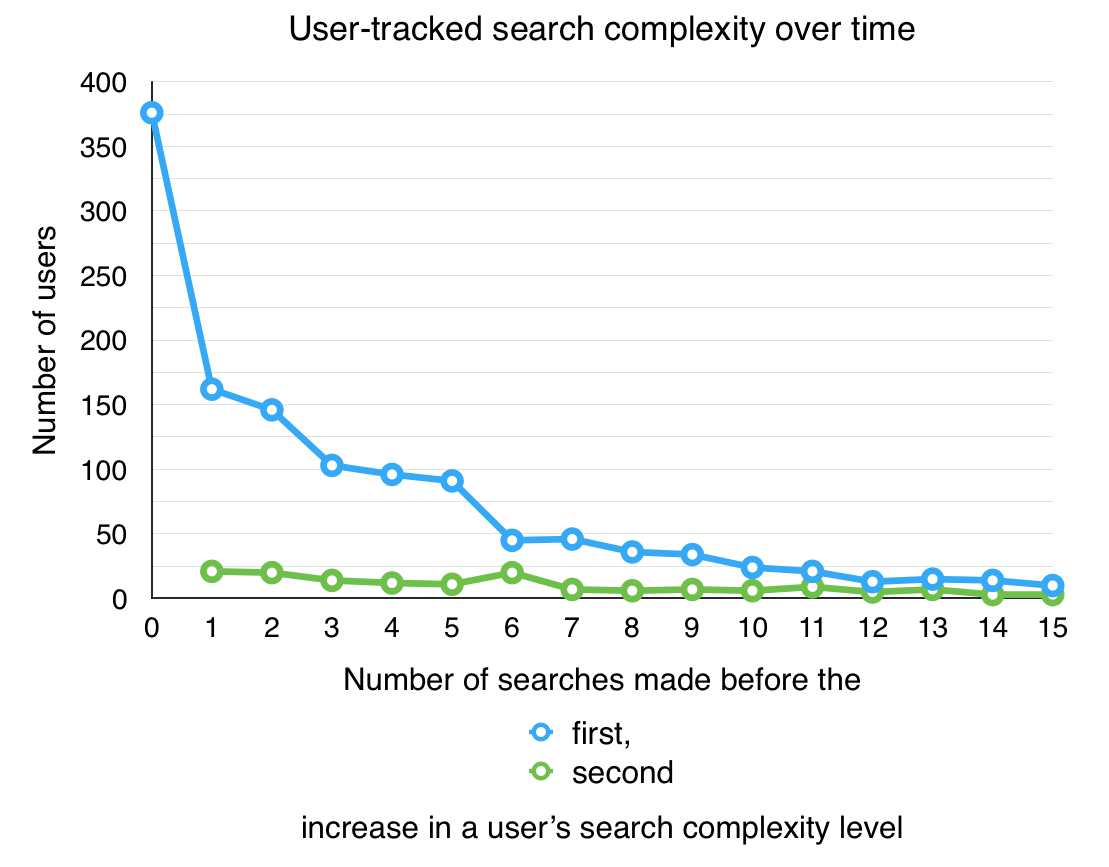
\includegraphics[width=1.00\textwidth]{images/graph/search_dt}

  \\
  \vspace{30pt}

  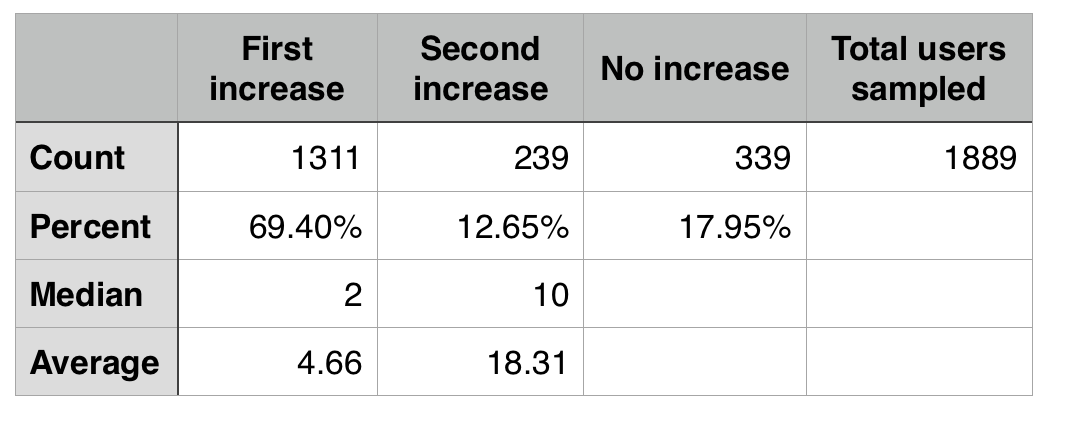
\includegraphics[width=0.65\textwidth]{images/table/search_dt}

  \caption{Etc}
  \label{fig:searchtypes}
\end{figure}

First increase 69.4\% of users), with a median of 2 searches.
Note that starting at search complexity one or greater counts as a ``searches before first increase value'' of 0.

Second increase (7.9\% of users)
Median: 8 searches
Average: 17.52 searches

DSQL++